\documentclass[10pt]{beamer}
\usepackage[utf8]{inputenc}
\usepackage{graphicx}
\usepackage{ragged2e}
\usepackage{listings}
\usepackage{minted}
\usepackage{multicol}
\usepackage {mathtools}
\usetheme{CambridgeUS}
\usecolortheme{dolphin}

% set colors
\definecolor{myNewColorA}{RGB}{0, 55, 158}
\definecolor{myNewColorB}{RGB}{0, 55, 158}
\definecolor{myNewColorC}{RGB}{0, 55, 158}
\setbeamercolor*{palette primary}{bg=myNewColorC, fg = white}
\setbeamercolor*{palette secondary}{bg=myNewColorB, fg = white}
\setbeamercolor*{palette tertiary}{bg=myNewColorA, fg = white}
\setbeamercolor*{titlelike}{fg=myNewColorA}
\setbeamercolor*{title}{bg=myNewColorA, fg = white}
\setbeamercolor*{item}{fg=myNewColorA}
\setbeamercolor*{caption name}{fg=myNewColorA}
\usefonttheme{professionalfonts}
\usepackage{natbib}
\usepackage{hyperref}

\newcommand{\specialcell}[2][c]{%
  \begin{tabular}[#1]{@{}c@{}}#2\end{tabular}}
  
\lstdefinelanguage{Kotlin}{
  comment=[l]{//},
  commentstyle={\color{gray}\ttfamily},
  emph={filter, first, firstOrNull, forEach, lazy, map, mapNotNull, println},
  emphstyle={\color{OrangeRed}},
  identifierstyle=\color{black},
  keywords={!in, !is, abstract, actual, annotation, as, as?, break, by, catch, class, companion, const, constructor, continue, crossinline, data, delegate, do, dynamic, else, enum, expect, external, false, field, file, final, finally, for, fun, get, if, import, in, infix, init, inline, inner, interface, internal, is, lateinit, noinline, null, object, open, operator, out, override, package, param, private, property, protected, public, receiveris, reified, return, return@, sealed, set, setparam, super, suspend, tailrec, this, throw, true, try, typealias, typeof, val, var, vararg, when, where, while},
  keywordstyle={\color{NavyBlue}\bfseries},
  morecomment=[s]{/*}{*/},
  morestring=[b]",
  morestring=[s]{"""*}{*"""},
  ndkeywords={@Deprecated, @JvmField, @JvmName, @JvmOverloads, @JvmStatic, @JvmSynthetic, Array, Byte, Double, Float, Int, Integer, Iterable, Long, Runnable, Short, String, Any, Unit, Nothing},
  ndkeywordstyle={\color{BurntOrange}\bfseries},
  sensitive=true,
  stringstyle={\color{ForestGreen}\ttfamily},
}

\setminted[kotlin]{
  linenos=true,
  breaklines=true,
  autogobble,
  encoding=utf8,
  fontsize=\footnotesize,
  frame=lines
}

\beamertemplatenavigationsymbolsempty
%------------------------------------------------------------
%\titlegraphic{\includegraphics[height=1.5cm]{download.png}} 

\setbeamerfont{title}{size=\large}
\setbeamerfont{subtitle}{size=\small}
\setbeamerfont{author}{size=\small}
\setbeamerfont{date}{size=\small}
\setbeamerfont{institute}{size=\small}
\title[]{DevOps per Applicazioni Mobile Multipiattaforma: un Caso di Studio Industriale}

\institute[]{Laboratorio di Sistemi Software}
\author[Filippo Paganelli]{Alma Mater Studiorum - Università di Bologna \\ Campus di Cesena}
\date[\textcolor{white}{A.A. 21/22}]
{
\begin{columns}[onlytextwidth]
    \begin{column}{0.5\textwidth}
        \begin{flushleft}
            Relatore:\\
            \textbf{Prof. Danilo Pianini}\\
            \vspace{3mm}
            Correlatore:\\
            \textbf{Prof.ssa Catia Prandi}
        \end{flushleft}
    \end{column}
        \begin{column}{0.5\textwidth}
        \begin{flushright}
            Presentata da:\\
            \textbf{Filippo Paganelli}
        \end{flushright}
    \end{column}
\end{columns}
\vspace{10mm}
A.A. 21/22 \\ III Sessione
}

%------------------------------------------------------------
%This block of commands puts the table of contents at the 
%beginning of each section and highlights the current section:
\AtBeginSection[]
{
  \begin{frame}
    \frametitle{Contents}
    \tableofcontents[currentsection]
  \end{frame}
}

%\AtBeginSection[]{
%  \begin{frame}
%  \vfill
%  \centering
%  \begin{beamercolorbox}[sep=8pt,center,shadow=true,rounded=true]{title}
%    \usebeamerfont{title}\insertsectionhead\par%
%  \end{beamercolorbox}
%  \vfill
%  \end{frame}
%}
%------------------------------------------------------------

\begin{document}

%The next statement creates the title page.
\frame{\titlepage}
%\begin{frame}
%\frametitle{Contents}
%\tableofcontents
%\end{frame}
%------------------------------------------------------------

% !TeX root = ../main.tex

\section{Introduzione}

\begin{frame}{Introduzione}
    \begin{columns}[onlytextwidth,t]
        \begin{column}{0.5\textwidth}
        
            \textbf{Necessità}:
            \begin{itemize}
                \item Innovazione
                \item Ottimizzazione
                \item Soddisfare i requisiti del cliente
                \item Tempi brevi di rilascio
                \item Accogliere le modifiche rapidamente
                \item Riuso del software
                \item Riduzione degli errori
                \item ...
            \end{itemize}
            
        \end{column}
        \begin{column}{0.5\textwidth}
        
            \textbf{Soluzione}:
            \begin{itemize}
                \item DevOps
                \item Applicazioni Multipiattaforma
            \end{itemize}
            
        \end{column}
    \end{columns}    
    
    \vspace{5mm}
    
    \textbf{Obiettivo}: Dimostrare l'efficacia della cultura DevOps e del paradigma multipiattaforma, adottati per lo sviluppo di applicazioni mobile
\end{frame}

\begin{frame}{DevOps}
    \begin{columns}[onlytextwidth]
        \begin{column}{0.45\textwidth}
        
            \textbf{Principi}:
            \begin{itemize}
                \item Comunicazione/Collaborazione
                \item Automazione
                \item Monitoraggio
            \end{itemize}
            
            \vspace{3mm}
            
            \textbf{Vantaggi}:
            \begin{itemize}
                \item Risparmio di tempo e risorse
                \item Tempi di consegna minori
                \item Maggiore qualità
            \end{itemize}
            
            \vspace{3mm}
            
            \textbf{Tecniche}:
            \begin{itemize}
                \item Continuous Integration
                \item Continuous Delivery
                \item Continuous Inspection
                \item ...
            \end{itemize}
            
        \end{column}
        \begin{column}{0.55\textwidth}
        
             \begin{figure}[H]
                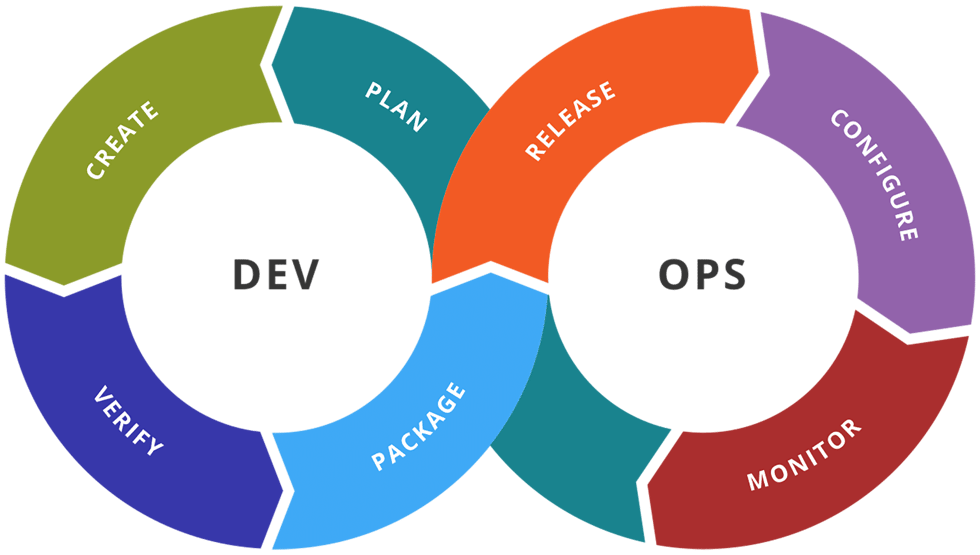
\includegraphics[width=1\textwidth]{img/Devops-toolchain.png}
            \end{figure}
            
        \end{column}
    \end{columns}
\end{frame}

\begin{frame}{Applicazioni Multipiattaforma}

    \textbf{Cross-piattaforma}:
    \begin{itemize}
        \item Condivisione/riuso totale del codice
        \item Performance limitate dovute alla presenza di uno strato software aggiuntivo di traduzione del codice
        \item Accesso limitato e con overhead alle funzionalità hardware del dispositivo dovuto alla presenza dello strato software aggiuntivo
        \item Frameworks: Ionic, Flutter, React Native, ...
    \end{itemize}
    
    \vspace{5mm}
    
    \textbf{Multi-piattaforma}:
    \begin{itemize}
        \item Condivisione/riuso della logica applicativa
        \item Performance elevate, equivalenti a quelle native
        \item Accesso completo e senza overhead alle funzionalità hardware del dispositivo
        \item Frameworks: \textbf{Kotlin Multiplatform Mobile}
    \end{itemize}
    
\end{frame}

\begin{frame}{Kotlin Multiplatform Mobile}
    \begin{columns}[onlytextwidth]
        \begin{column}{0.55\textwidth}
        
             \begin{figure}[H]
                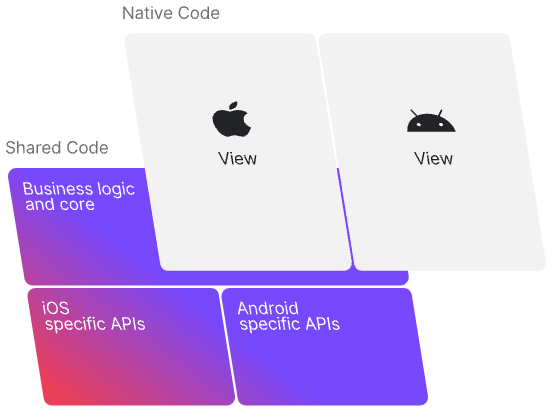
\includegraphics[width=1\textwidth]{img/kmm-stack-official.png}
            \end{figure}
            
        \end{column}
        \begin{column}{0.45\textwidth}
        
            \textbf{Caratteristiche}:
            \begin{itemize}
                \item Framework per lo sviluppo di applicazioni mobile multipiattaforma per Android e iOS
                \item Ancora non molto maturo (fase ``pre-stable'')
                \item Utilizzato in produzione da aziende come Netflix, Philips e VMware
                \item Il codice condiviso viene compilato in binari eseguibili direttamente dal dispositivo senza il bisogno di strati software aggiuntivi
            \end{itemize}
            
        \end{column}
    \end{columns}
\end{frame}
% !TeX root = ../main.tex

\section{Caso di Studio}

\begin{frame}{Contesto Aziendale}
    \begin{figure}[H]
        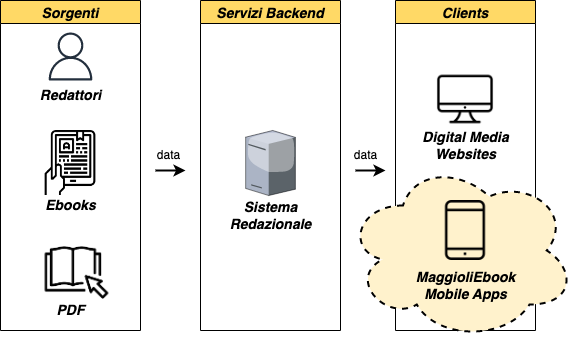
\includegraphics[width=0.7\textwidth]{img/contesto-aziendale.png}
    \end{figure}
    \begin{itemize}
        \item \textbf{Core Business}: Editoria e servizi per la pubblica amministrazione e professionisti
        \item \textbf{Necessità}: Sviluppare un nuovo metodo di accesso alle pubblicazioni digitali che sia più accessibile e pratico
        \item \textbf{Dominio}: Editoria digitale
    \end{itemize}
\end{frame}

\begin{frame}{Requisiti: Processo}
    \begin{figure}[H]
        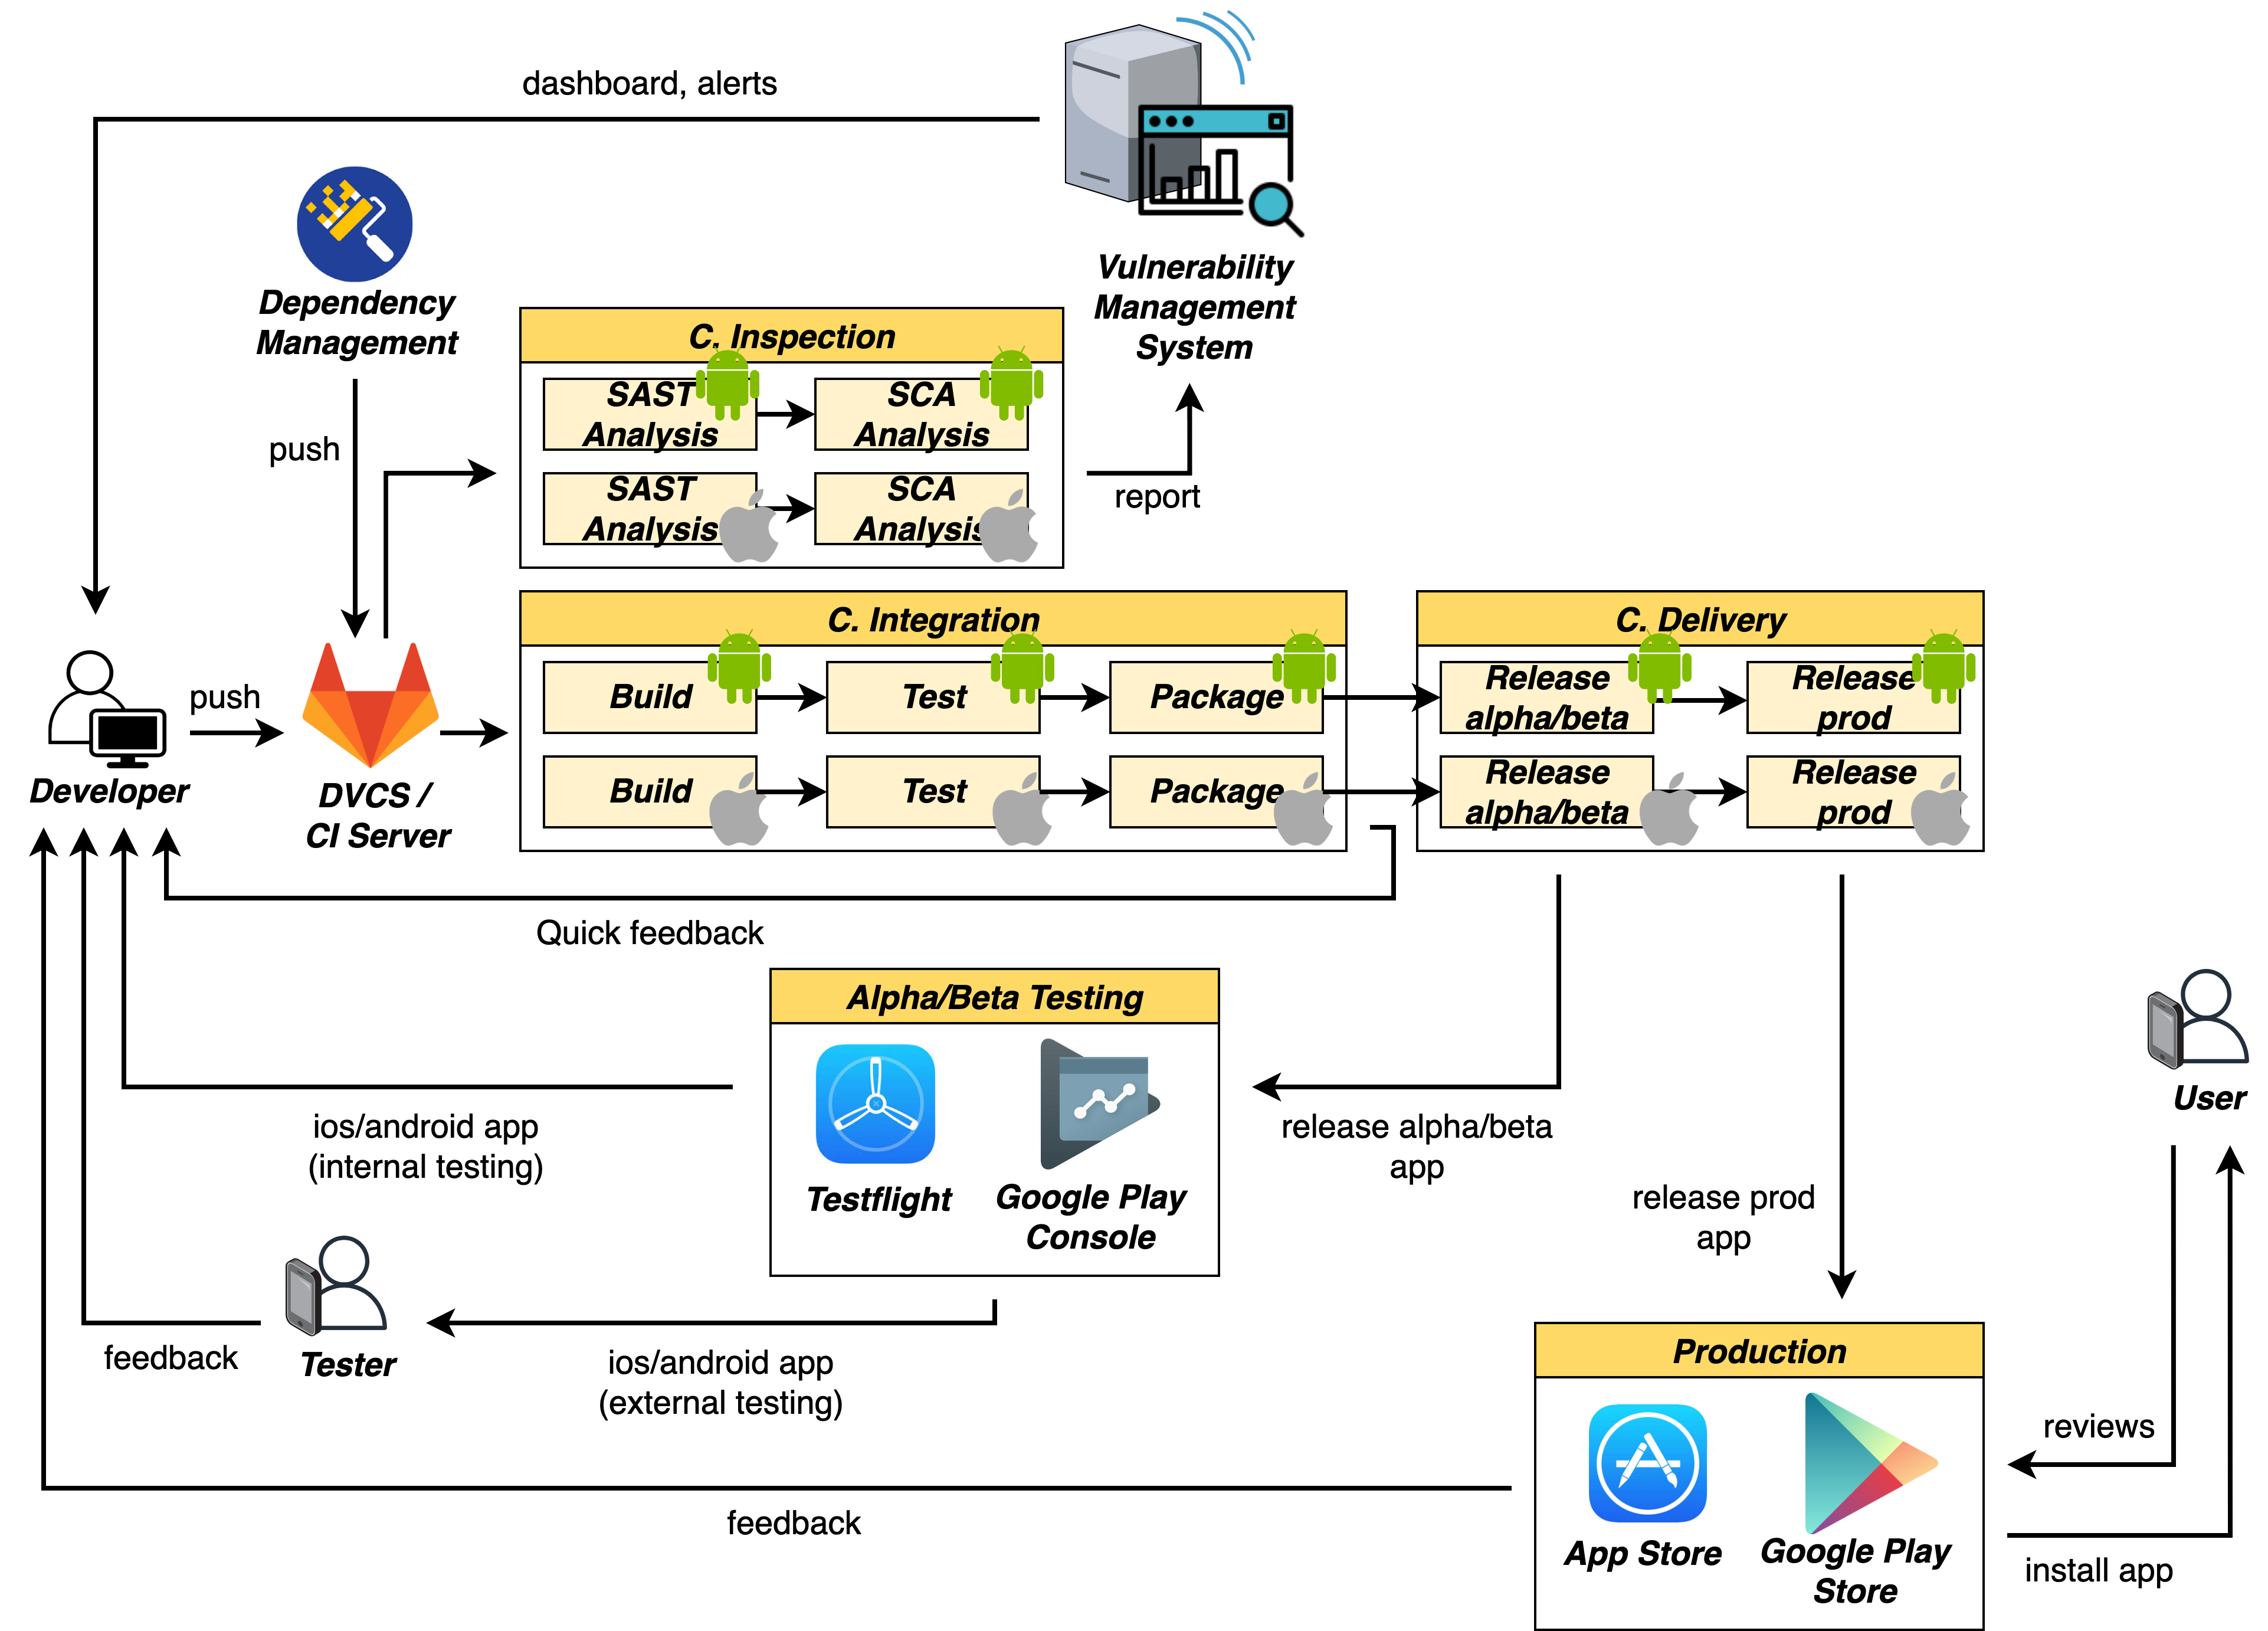
\includegraphics[width=0.89\textwidth]{img/full-cicd.png}
    \end{figure}
\end{frame}

\begin{frame}{Requisiti: Applicazione}
    \begin{columns}[onlytextwidth]
        \begin{column}{0.5\textwidth}
            \textbf{Tipologia}: E-Reader\\
            \vspace{5mm}
            \textbf{Funzionali}:
            \begin{itemize}
                \item Visualizzazione contenuti digitali
                \item Portabilità e leggibilità
                \item Ricerca pubblicazioni in base all'abbonamento dell'utente
                \item Personalizzazione tramite segnalibri e annotazioni
                \item Gestione preferiti
            \end{itemize}
            \vspace{5mm}
            \textbf{Tecnologici}:
            \begin{itemize}
                \item Versione Android e iOS
                \item Kotlin Multiplatform Mobile
            \end{itemize}
        \end{column}
        \begin{column}{0.45\textwidth}
             \begin{figure}[H]
                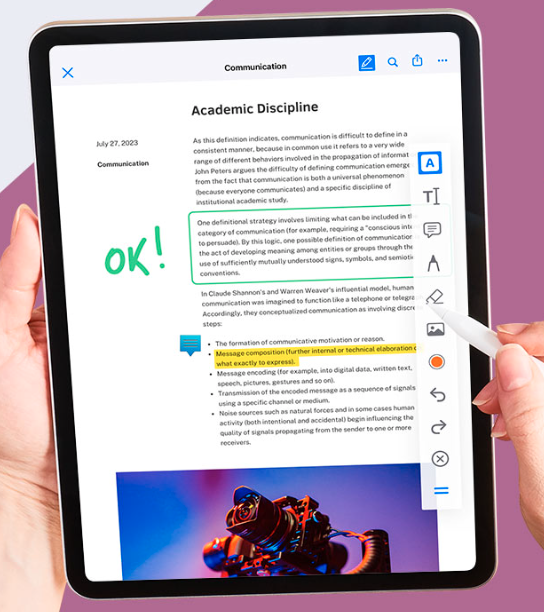
\includegraphics[width=1\textwidth]{img/e-reader.png}
            \end{figure}
        \end{column}
    \end{columns}
\end{frame}
% !TeX root = ../main.tex

\section{Automazione del Processo di Sviluppo}

\begin{frame}{Flusso di Lavoro}
    \begin{columns}[onlytextwidth]
        \begin{column}{0.95\textwidth}
            \begin{figure}[H]
                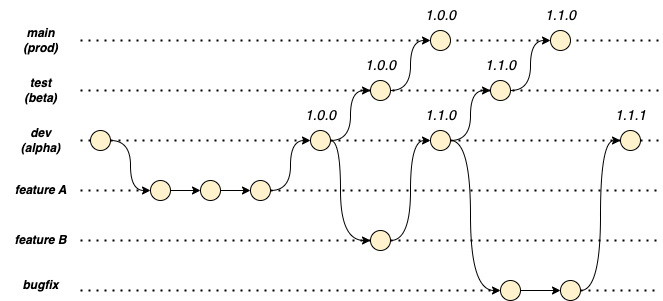
\includegraphics[width=0.9\textwidth]{img/branching-model.png}
            \end{figure}
        \end{column}
        \begin{column}{0.05\textwidth}
        \end{column}
    \end{columns}
    \vspace{5mm}
    \begin{columns}[onlytextwidth]
        \begin{column}{0.4\textwidth}
            \textbf{Branch principali}:
            \begin{itemize}
                \item dev
                \item test
                \item main
            \end{itemize}
        \end{column}
        \begin{column}{0.4\textwidth}
            \textbf{Ambienti}:
            \begin{itemize}
                \item Testing interno (alpha)
                \item Testing esterno (beta)
                \item Produzione (prod)
            \end{itemize}
        \end{column}
    \end{columns}
\end{frame}

\begin{frame}{Continuous Integration/Delivery}
    \vspace{3mm}
    \begin{columns}[onlytextwidth]
        \begin{column}{0.45\textwidth}
            \textbf{Continuous Integration}
            \vspace{2mm}
            \begin{itemize}
                \item \textbf{Principio}: Integrazione frequente di piccole modifiche, testate automaticamente
                \vspace{2mm}
                \item \textbf{Stages}:
                \begin{itemize}
                    \item Build
                    \item Test
                    \item Package
                \end{itemize}
            \end{itemize}
        \end{column}
        \begin{column}{0.45\textwidth}
            \textbf{Continuous Delivery}:
            \vspace{2mm}
            \begin{itemize}
                \item \textbf{Principio}: Rilascio frequente di piccole modifiche o funzionalità, eseguito in modo automatico
                \vspace{2mm}
                \item \textbf{Stages}:
                \begin{itemize}
                    \item Release alpha
                    \item Release beta
                    \item Release prod
                \end{itemize}
            \end{itemize}
        \end{column}
    \end{columns}
    \begin{figure}[H]
        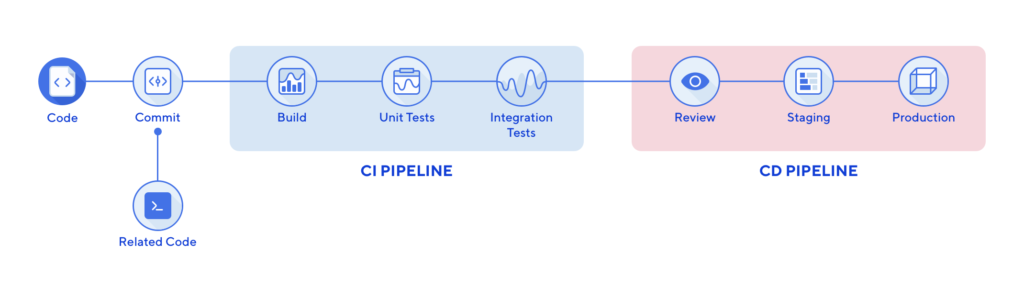
\includegraphics[width=1\textwidth]{img/ci-cd-pipeline.png}
    \end{figure}
\end{frame}

\begin{frame}{Continuous Inspection}
        \begin{columns}[onlytextwidth]
        \begin{column}{0.45\textwidth}
            \textbf{Continuous Inspection}
            \vspace{2mm}
            \begin{itemize}
                \item \textbf{Principio}: Analisi automatica del codice per garantire un certo livello di qualità e di sicurezza
                \vspace{2mm}
                \item \textbf{Stages}:
                \begin{itemize}
                    \item SAST (Static Application Security Testing)
                    \item SCA (Software Composition Analysis)
                \end{itemize}
            \end{itemize}
        \end{column}
        \begin{column}{0.5\textwidth}
            \begin{figure}[H]
                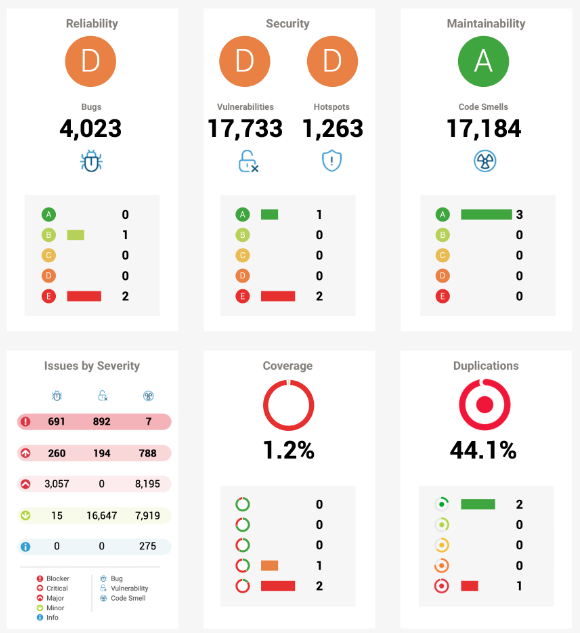
\includegraphics[width=1\textwidth]{img/sonar-screenshot.png}
            \end{figure}
        \end{column}
    \end{columns}
\end{frame}

\begin{frame}{Sistema Obiettivo}
    \begin{figure}[H]
        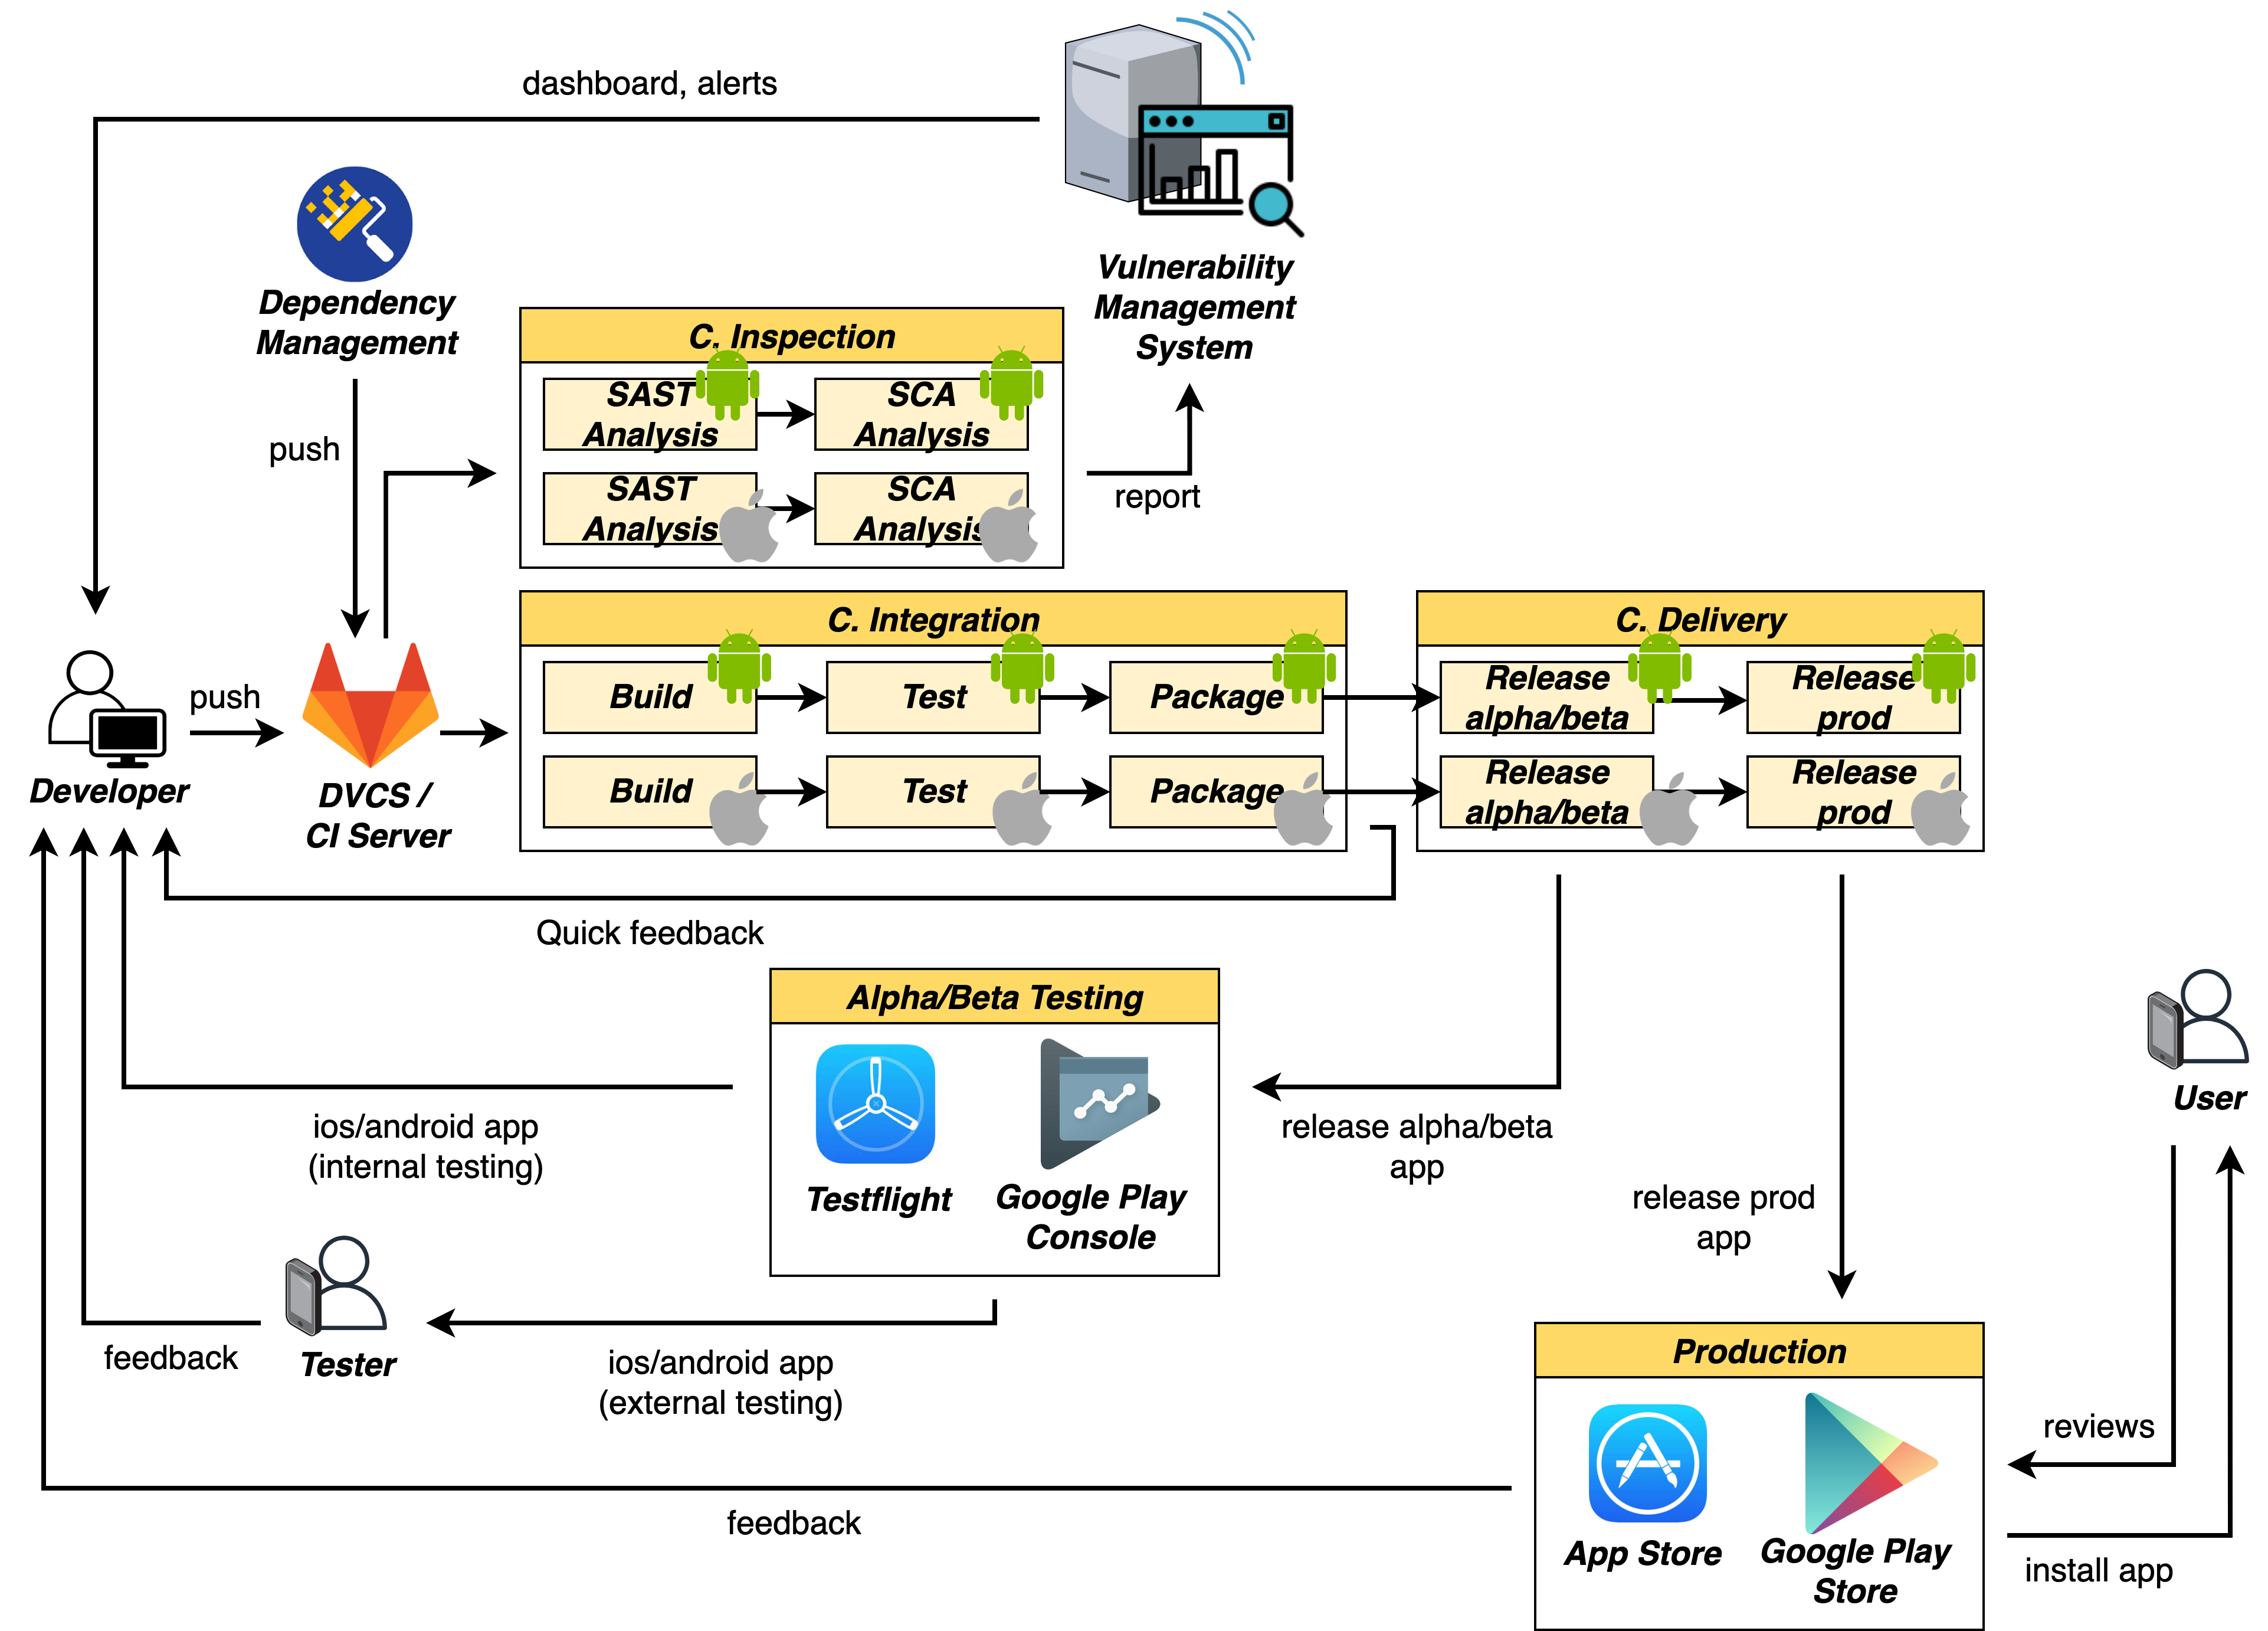
\includegraphics[width=0.89\textwidth]{img/full-cicd.png}
    \end{figure}
\end{frame}
% !TeX root = ../main.tex

\section{Sviluppo Applicazione}

\begin{frame}{Processo di Sviluppo}
    \begin{columns}[onlytextwidth]
        \begin{column}{0.4\textwidth}
            \textbf{Progettazione}:
            \begin{itemize}
                \item Modellazione dominio (editoria digitale)
                \item Progettazione UX/UI
                \item Definizione architettura
            \end{itemize}
            \vspace{3mm}
            \textbf{Implementazione}:
            \begin{itemize}
                \item Ricerca Librerie
                \item Sviluppo logica applicativa (modulo condiviso)
                \item Sviluppo UI Android
                \item Sviluppo UI iOS
            \end{itemize}
        \end{column}
        \begin{column}{0.6\textwidth}
             \begin{figure}[H]
                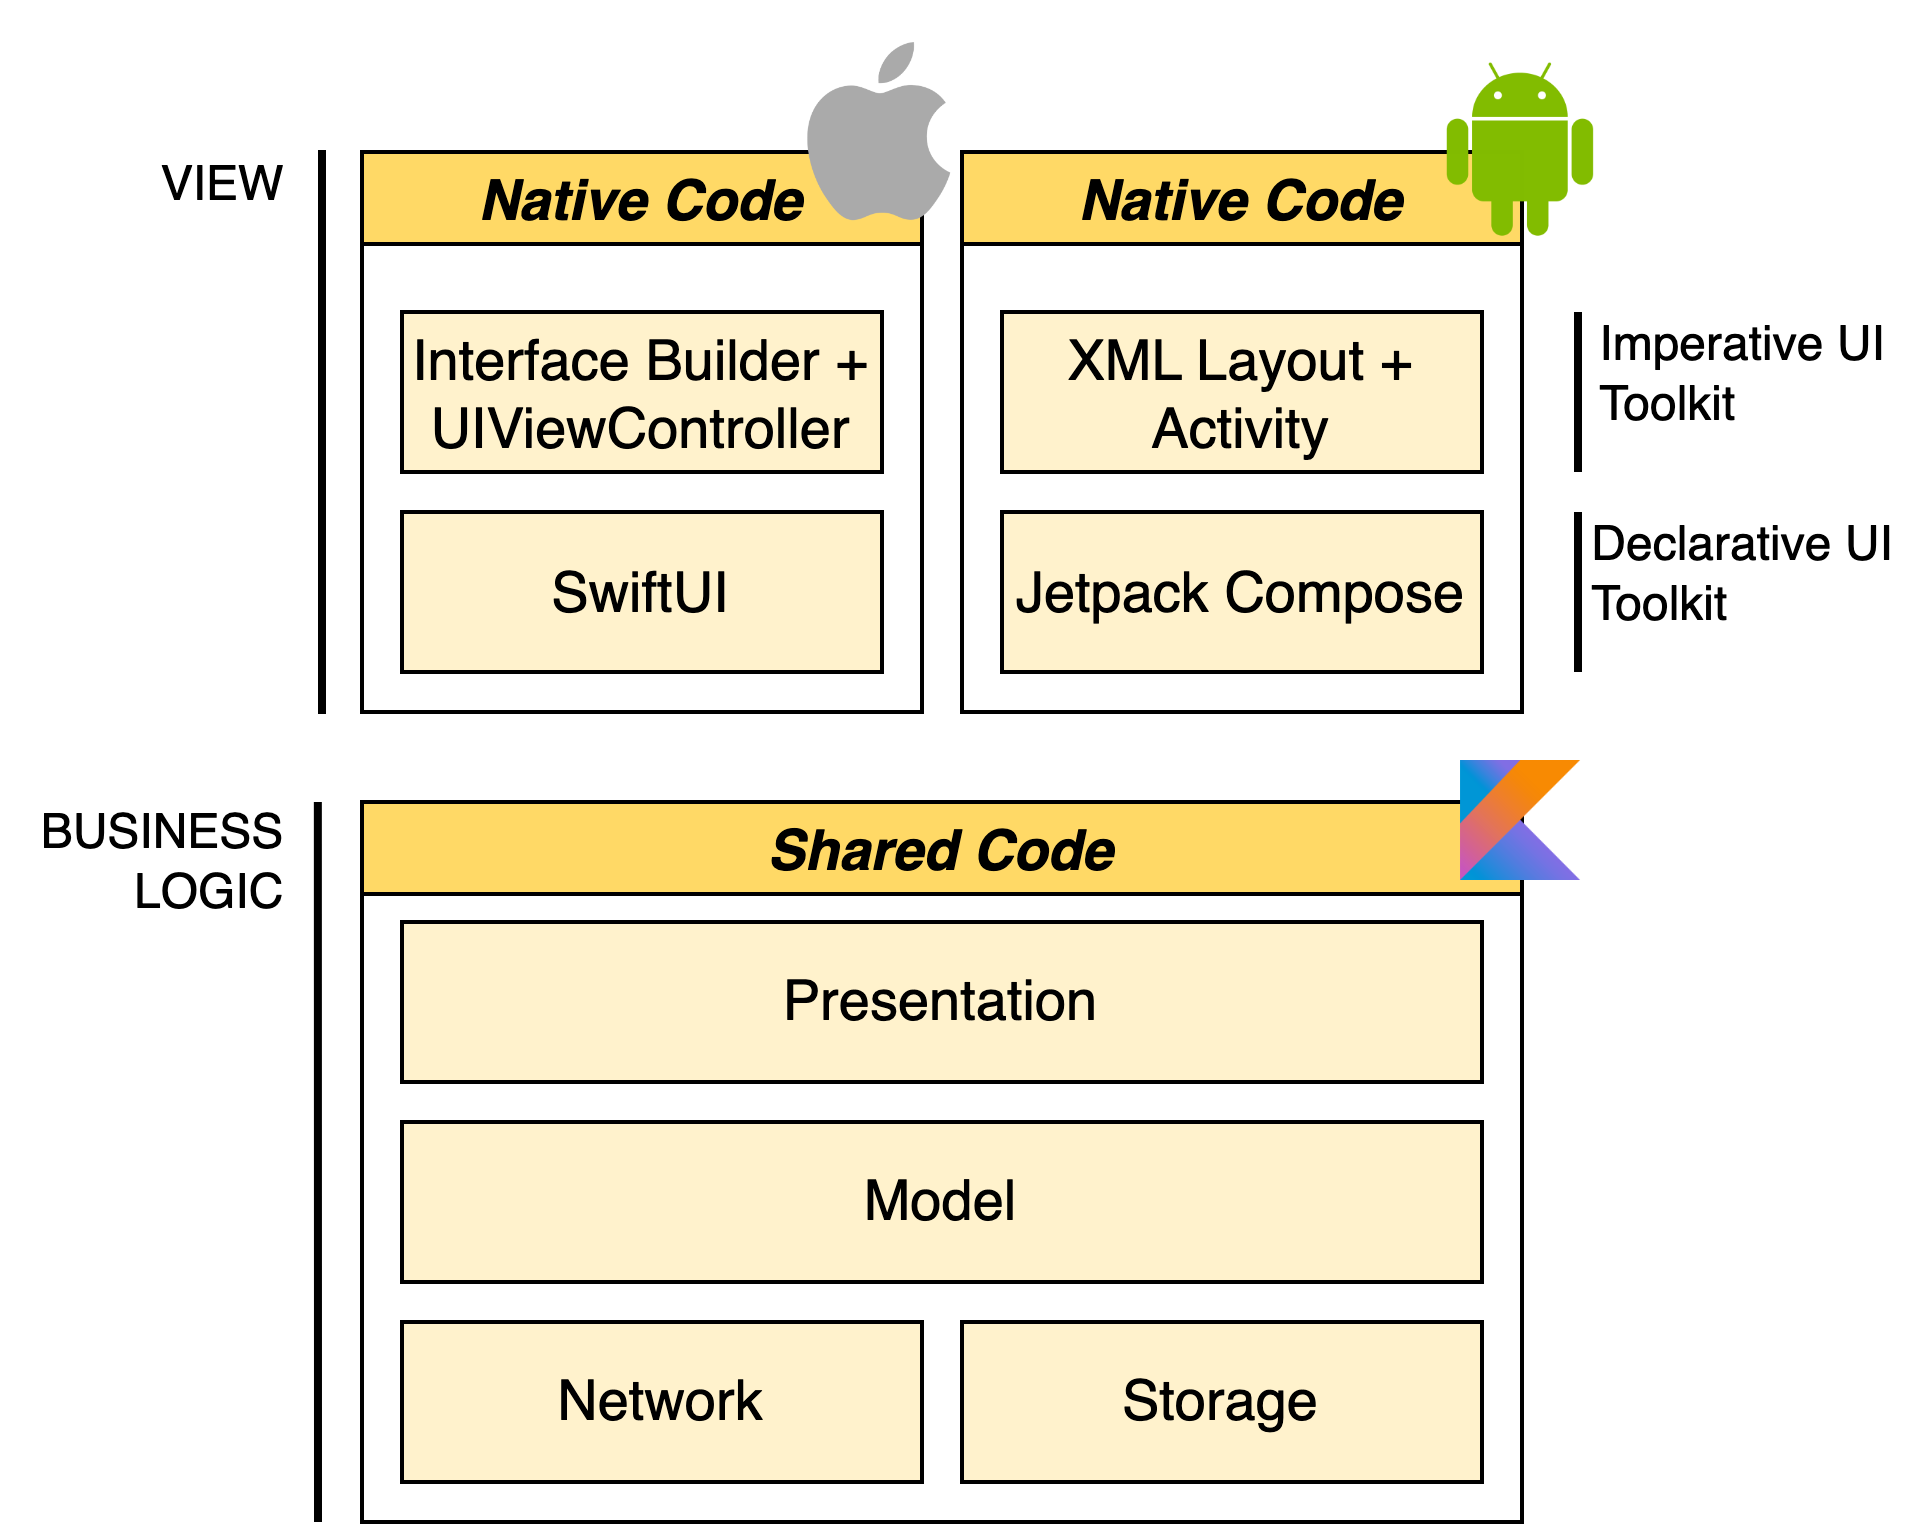
\includegraphics[width=1\textwidth]{img/stack_kmm.png}
            \end{figure}
        \end{column}
    \end{columns}
\end{frame}

\begin{frame}{Logica Applicativa}
    
\end{frame}

\begin{frame}{UI Android}
    
\end{frame}

\begin{frame}{UI iOS}
    
\end{frame}
% !TeX root = ../main.tex

\section{Conclusioni}

\begin{frame}{Conclusioni}

    \textbf{Risultati raggiunti}:
    \begin{itemize}
        \item Breve time-to-market
        \item 3 mesi da inizio sviluppo a distribuzione applicazione, sia Android che iOS
        \item 28 minuti (media) dalla modifica del codice al rilascio, sia Android che iOS
        \item Framework Kotlin Multiplatform non ancora maturo per scenari molto complessi
    \end{itemize}

    \vspace{3mm}

    \textbf{Lavori futuri}:
    \begin{itemize}
        \item Realizzazione stesso caso di studio con metodologia crosspiattaforma
        \item Confronto multipiattaforma vs crosspiattaforma
        \item Monitoraggio applicazione e utente
    \end{itemize}
    
\end{frame}


\begin{frame}
    \begin{center}
        \LARGE Grazie dell'attenzione
    \end{center}
\end{frame}

\end{document}